%----------------------------------------------------------------------------
%
%	This template was created by
%		Christian Krieg <christian.krieg@alumni.tuwien.ac.at>
%
%	April 2018
%
%----------------------------------------------------------------------------
%
\documentclass[%
	a4paper,
]
{article}
%
%----------------------------------------------------------------------------
%
% Institution
%
%\institution{Institute of Computer Technology}
%
%----------------------------------------------------------------------------
%
% Use the 'Libertine' font type
%
\usepackage{libertine}
\usepackage[T1]{fontenc}
\usepackage[utf8]{inputenc}
%
%----------------------------------------------------------------------------
%
% Set page margins
%
\usepackage{geometry}
\geometry{%
	left   = 2cm,
	right  = 2cm,
	top    = 2cm,
	bottom = 2cm
}
%
%----------------------------------------------------------------------------
%
% Set line spacing
%
\usepackage{setspace}
\setstretch{1}
%
%----------------------------------------------------------------------------
%
% Settings for hyperlinks
%
\usepackage{hyperref}
\hypersetup{%
	colorlinks = true,
	allcolors  = blue,
}
%
%----------------------------------------------------------------------------
%
% Use colors
%
\usepackage{xcolor}
\usepackage{colortbl}
%
%----------------------------------------------------------------------------
%
% Define a TODO and a DONE command
%
\newcommand{\todo}[1]{\textcolor{red}{#1}}
\newcommand{\done}[1]{}
%
%----------------------------------------------------------------------------
%
% Use glossaries
%
\usepackage{glossaries}
\makeglossaries
%
% Glossary entries
%
\newglossaryentry{hdl}{
  name={HDL},
  description={Hardware description language},
  text={HDL},
  first={hardware description language (HDL)},
  plural={HDLs},
  firstplural={hardware description languages (HDLs)},
}


\newglossaryentry{fpga}{
	name = {FPGA},
	description = {Field-programmable gate array},
	text = {FPGA},
	first = {field-programmable gate array (FPGA)},
	plural = {FPGAs},
	firstplural = {field-programmable gate arrays (FPGAs)},
}
%
%
%\newglossaryentry{}{
%  name={},
%  description={},
%  text={},
%  first={},
%  plural={},
%  firstplural={},
%}
%
%----------------------------------------------------------------------------
%
% Settings for citations and the bibliography
%
\usepackage[%
	backend     = biber,
	maxbibnames = 99,
	autocite    = footnote,
	citestyle   = verbose-ibid,
	firstinits=true,
]{biblatex}
\bibliography{bib/report}
%
%----------------------------------------------------------------------------
%
%	TikZ -- TikZ ist kein Zeichenprogramm
%
\usepackage{tikz}
\usepackage{tikz-timing}
\usepackage{etoolbox}
\usetikzlibrary{mindmap}
\usetikzlibrary{shapes}
\usetikzlibrary{arrows}
\usetikzlibrary{decorations}
\usetikzlibrary{shapes.symbols}
\usetikzlibrary{shapes.geometric}
\usetikzlibrary{shapes.multipart}
\usetikzlibrary{positioning}
\usetikzlibrary{patterns}
\usetikzlibrary{calc}
\usetikzlibrary{scopes}         % cf. pgfmanual p.66
\usetikzlibrary{chains}         % cf. pgfmanual p.284
\usetikzlibrary{fit}
\usetikzlibrary{matrix}
\usetikzlibrary{decorations}
\usetikzlibrary{circuits.logic}
\usetikzlibrary{circuits.logic.IEC}
\usetikzlibrary{shapes.gates.logic.IEC}
\usetikzlibrary{circuits.logic.US}
\usetikzlibrary{shapes.gates.logic.US}
\usetikzlibrary{circuits.ee}
\usetikzlibrary{circuits.ee.IEC}
\usetikzlibrary{backgrounds}
\usetikzlibrary{automata}
\usetikzlibrary{intersections}
\usetikzlibrary{plotmarks}
\usepgflibrary{fpu}
\usetikzlibrary{decorations.pathreplacing}
%
%----------------------------------------------------------------------------
%
% TikZ shapes
%  
	\input{lib/tikz/dff}
%
%----------------------------------------------------------------------------
%
% Use AMS math fonts
%
\usepackage{amsfonts}
\usepackage[sans]{dsfont}
%
%----------------------------------------------------------------------------
%
% Use multiple figures in one float
%
\usepackage{subcaption}
%
%----------------------------------------------------------------------------
%
% Use dummy text
%
\usepackage{lipsum}
%
%----------------------------------------------------------------------------
%
% Use extended list environments (e.g., 'inparaenum')
%
\usepackage{paralist}
%
%----------------------------------------------------------------------------
%
% Use listings
%
\usepackage{listings}

\lstdefinestyle{customc}{
  belowcaptionskip=1\baselineskip,
  breaklines=true,
  frame=single, numbers=left,
  xleftmargin=\parindent,
  language=C,
  showstringspaces=false,
  basicstyle=\footnotesize\ttfamily,
  keywordstyle=\bfseries\color{green!40!black},
  commentstyle=\itshape\color{purple!40!black},
  identifierstyle=\color{blue},
  stringstyle=\color{orange},
}
\lstdefinestyle{vhdl}
{
	language=VHDL,
  basicstyle=\linespread{1}\scriptsize\ttfamily\color{black},
  commentstyle=\scriptsize\itshape,
  escapeinside={(*@}{@*)},
  frame=single, numbers=left,
%  numbersep=5pt,
  xleftmargin=15pt,
  xrightmargin=5pt,
  numbersep=5pt,
  breaklines=true,
  moredelim=**[is][\ttfamily\bfseries\color{red}]{(*}{*)},
}

\lstdefinestyle{verilog}
{
	language=Verilog,
  basicstyle=\linespread{1}\scriptsize\ttfamily\color{black},
  commentstyle=\scriptsize\itshape,
  escapeinside={(*@}{@*)},
  frame=single, numbers=left,
%  numbersep=5pt,
  xleftmargin=15pt,
  xrightmargin=5pt,
  numbersep=5pt,
  breaklines=true,
  moredelim=**[is][\ttfamily\bfseries\color{red}]{(*}{*)},
}
%
%----------------------------------------------------------------------------
%
% Typeset pseudo code
%
\usepackage{syntax}
%
%----------------------------------------------------------------------------
%
% More options for boxes
%
\usepackage{realboxes}
%
% Command for vertical text in tabulars
%
\newcommand*\rot{\rotatebox{90}}
%
%----------------------------------------------------------------------------
%
% Use \textsubscript
%
%\usepackage{fixltx2e}
%
%----------------------------------------------------------------------------
%
% More options for tabulars
%
\usepackage{array}
%
%----------------------------------------------------------------------------
%
% Use appendices
%
\usepackage[titletoc]{appendix}
%
%----------------------------------------------------------------------------
%
% Use the cleverref package -- Load this package as the very last!
%
\usepackage{cleveref}
%
%----------------------------------------------------------------------------
%
%
%----------------------------------------------------------------------------
%
% Document body
%
\begin{document}
%
%----------------------------------------------------------------------------
%
\begin{titlepage}

	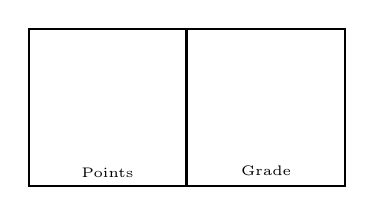
\begin{tikzpicture}[thick]
		\node (points) at (0,0) [draw,minimum size=2cm] {};
		\node (lbl-points) at (points.south) [anchor=south,font=\tiny] {Points};
		\node (grade) at (points.east) [draw,minimum size=2cm,anchor=west,
			outer sep=0] {};
		\node (lbl-grade) at (grade.south) [anchor=south,font=\tiny] {Grade};
	\end{tikzpicture}

	\begin{flushright}

		% Update this with your team number
		\huge\bfseries
		Team: 6 \\[1em]

		% Update this with your matriculation number, first name, second name
		\large
		01228774 Constantin SCHIEBER \#1	\\
		0122576 Petar KOSIC \#2	\\
	
	\end{flushright}

	\vspace{5em}

	\begin{center}
		{\huge Digital Integrated Circuits Lab (LDIS)}\\[1em]
		{\Large 384.088, Summer Term 2018} \\[2em]
		{\large Supervisors:\\[.5em]
			Christian Krieg, Martin Mosbeck, Axel Jantsch} \\[10em]

		{\Huge Task 2: Implementing Argon2}\\[10em]
	\end{center}


	\begin{abstract}

		Parts of a key derivation function (KDF) - Argon2 - had to be implemented and integrated
with implementations of other groups. The result of this task is a working KDF that can be
reused.

A Permutation function, a compression function and a truncation function and the
verification process are subsequently presented in this work.


	\end{abstract}

\end{titlepage}
%
%----------------------------------------------------------------------------
%
\section{Problem statement and motivation}
\label{sec:problem}

A \gls{trng} based on the paper from \autocite{Majzoobi2011} had to be implemented.

The paper shows an approach that promises a resource efficient and fast solution to the
problem of generating long enough keys for cryptographic algorithms. The reproduction of
the results in the paper is a challenging and important task, as the paper is very
incomplete regarding information about the actual implementation.

The source of randomness is based on the metastability characteristics of a d-flipflop when violating setup or hold times of the flipflop.
To create such violations the novel approach of delay lines is introduced. The data and
clock input ports of the flipflop are both preceded by a series of \glspl{lut} blocks. 
These \glspl{lut} blocks are functionally just used as inverters - but due to the
inner structe of a \glspl{lut} a delay can be introduced by applying different control
signals to the \glspl{lut} ports.


%
%----------------------------------------------------------------------------
%
\section{Implementation (proposed solution)}
\label{sec:solution}

Some decisions regarding all parts of the implementation were made to provide a
solution that works in simulation at least. These assumptions do not conform to the specification.

\begin{enumerate}
\item Grade of achieveable parallelism is 1
\item Design is not synthesizable and ignores especially the low area criteria
\item Simulation only possible with VHDL-2008 Standard, --std=08 flag mandatory
\end{enumerate}

\subsection{Truncation Function trunc(a)}
The truncation function trunc(a) is implemented as a vhdl function in a package aswell as a
fully fledged component. Our design uses the function, which is located in the
permutate_pkg.vhd, due to its easier usage in sequential code (aka in processes).
\subsection{Permutation Function P}
The permutation function P was also implemented as a vhdl component at first.
Due to the heavy usage of sequential code segments a redesign to a vhdl function was 
done. It resides now in the permutate_pkg.vhd.
The implementation is as suggested by the \autocite{irtf-draft} - but heavily sequential.
One could implement a more elegant solution that allows for parallelization of round
function GB calls that are independet of each other (note that not all calls are
independet, as they operate on the same matrix). 
\subsubsection{Round Function GB}
The round function GB doesn't have its own section but is the foundation of all other
functionalities. 
Yet again it was implemented firstly as a component, only to be translated to a function,
which also resides in the permutate_pkg.vhd. 
It is implemented straight forward as specified.

\subsubsection{Verification}
As the round function represents a vital part of the implementation, the generation of
good test cases was a main goal. To achieve this goal the code of the C reference solution
\autocite{argon2-github}
was analyzed and altered.
The extraction of test vectors at key points of the operation was planned at several parts
of the argon2 implementation, including the following files from the /src directory:

\begin{itemize}
\item ref.c
\item blake2blake2b.c
\item blake2blamka-round-ref.h
\item ..Makefile
\end{itemize}


Extraction of the test vectors from the code was done by simple tagged printfs
of the UINT64 data blocks. The blocks were printed in decimal for simplicity and further
processing (see \Cref{lst:blake2bc}). Removal of the tags was done by hand, a python script (convert_binary.py) then parses the blocks and converts them into their binary representation.

\begin{lstlisting}[
	style = customc,
	caption = {Suboptimal extraction point in blake2b.c},
	label = lst:blake2bc,
]
		...
		...
#define ROUND(r)                       	
    do {                                	
		printf("INPUTSTART\n");			   	
		for (i = 0; i < 16; i++) {		   	
			printf("%" PRIu64 "\n", v[i]); 	
		}								   	
		printf("INPUTEND\n");			   	
		G(v[0], v[4], v[8], v[12]);        
		G(v[2], v[6], v[10], v[14]);    
		...
		...
		printf("OUTPUTSTART\n");			   	
		for (i = 0; i < 16; i++) {		   	
			printf("%" PRIu64 "\n", v[i]); 	
		}								   	
		printf("OUTPUTSTART\n");			   	

\end{lstlisting}

First tests proved to be unsuccessful though, as the implementation of the permutation
function in the C Code differs from the one proposed in the irtf-draft\autocite{irtf-draft}.
To double check on our proposed solution a python script that also implements the
permutation P and round GB function was created.

The python and vhdl implementations did deliver the same output. Analyzing the reference
solution more closely revealed that there are reference, optimized and actually used code
lines that rely heavily on preprocessor statements. 

Analysis of the Makefile showed, that a check for the platform was done (\Cref{lst:makefile}), and if the
platform was supported the optimized version of the files was used.
After modifying the Makefile accordingly (and now actually using the reference solution)
the generated output \textbf{did} match the output of our vhdl solution, see also table
\Cref{tbl:permresults}.

\begin{lstlisting}[
	style = customc, 
	caption = {Parameters for the argon2 execution},
	label = lst:RunArgon,
]
echo -n "password" | ./argon2 somesalt -t 1 -m 16 -p 1 -l 24
\end{lstlisting}

\begin{lstlisting}[
	style = customc,
	caption = {Makefile, deactivate optimizations},
	label = lst:makefile,
]

OPTTEST := $(shell $(CC) -Iinclude -Isrc -march=$(OPTTARGET) src/opt.c -c \
			-o /dev/null 2>/dev/null; echo $$?)
# Detect compatible platform
ifneq ($(OPTTEST), 0)
$(info Building without optimizations)
	SRC += src/ref.c
else
$(info Building with optimizations for $(OPTTARGET))
	CFLAGS += -march=$(OPTTARGET)
	SRC += src/opt.c
endif
\end{lstlisting}

\begin{table}[ht]
	\centering
	\caption{Permutation Function P Outputs}
	\label{tbl:permresults}
	\begin{tabular}{c|cccc}
	\hline
	Input & Python3.5 & VHDL & C Reference & C Actual \\ 
	\hline
	 6A09E667F2BDC948 & 4B86FAA34237F816 & 4B86FAA34237F816 & 4B86FAA34237F816 & 3D9D014CA238A25D \\  
	 510E527FADE682D1 & 826371B4B7CF06DB & 826371B4B7CF06DB & 826371B4B7CF06DB & D9CE83A69663A233 \\
	 6A09E667F3BCC908 & 6915F3A835F68E52 & 6915F3A835F68E52 & 6915F3A835F68E52 & B8023558C91686D7 \\  
	 510E527FADE682E9 & 4A645E346BE317D8 & 4A645E346BE317D8 & 4A645E346BE317D8 &
	 2E207F7532A740EC \\
	 \hline
	\end{tabular}
\end{table}

For one part the upper half of the 128 Byte Input is initialized in an unexpected way that
is not mentioned in the \autocite{irtf-draft}. This seems to be part of the regular way of
implementing blake2b, see the code listing \Cref{lst:blake2bcRound} where v[15] is initialized
by loading a fixed UINT64 and XORing it with an unknown parameter f[1]. 

\begin{lstlisting}[
	style = customc,
	caption = {Differing implementation of Round Function},
	label = lst:blake2bcRound,
]
/*Strange Vector Init*/ v[15] = blake2b_IV[7] ^ S->f[1];
	...
	...
#define G(r, i, a, b, c, d)                                                   
    do {                                                                       
        a = a + b + m[blake2b_sigma[r][2 * i + 0]];                            
        d = rotr64(d ^ a, 32);                                                 
        c = c + d;                                                             
        b = rotr64(b ^ c, 24);                                                 
\end{lstlisting}


When using the correct test vectors from the reference function or our own
generated test vectors from the python script the permutation function shows correct
behaviour.


\subsection{Compression Function G}
\subsection{Argon2, Steps 5-8}


%\begin{lstlisting}[
%	style = vhdl,
%	caption = {},
%	label = lst:,
%]
%\end{lstlisting}



%
%----------------------------------------------------------------------------
%
\section{Results (verification plan)}
\label{sec:results}

The goal of implementing a working \gls{trng} was not reached during this lab assignment. 

The number generation was extremely deterministic, as the p-values obtained by the NIST Test
Suite score all a 0. The Test Suite (and also its wrapper) throw many igamc: UNDERFLOW
errors that were at first wrongfully interpreted as errors due to the used compiler and
the used math libraries. 
After further investigation this just means that the p-value is so low that an exception
is thrown and the p-value gets replaced by 0. 

As a good p value should be around 0.5 (equal chance of guessing and not guessing the
correct sequence) the conclusion must be drawn that the numbers are not suitable for
cryptography at all. 

Interestingly enough a run with the dieharder test suite yields good results on the same
data. Further investigation is needed on the why.

\begin{table}[htp]
	\centering
	\caption{Dieharder results for experiment TRNG}
	\label{tbl:results}
	\begin{tabular}{lccc}

		\hline
		\textbf{Test} & \textbf{tSample} &\textbf{P-value} &\textbf{Passed} \\
		\hline
         sts_monobit&       100000&     0.18544306&  PASSED  \\ 
            sts_runs&       100000&     0.95997337&  PASSED  \\
          sts_serial&       100000&     0.13818581&  PASSED  \\
          sts_serial&       100000&     0.99575888&   WEAK   \\
		\hline
	\end{tabular}

\end{table}
\begin{table}[htp]
	\centering
	\caption{NIST-STS results for experiment XYZ}
	\label{tbl:NISTresults}
	\begin{tabular}{lc}

		\hline
		\textbf{Test} & \textbf{P-value} \\
		\hline

		Frequency & 0.0\\
		Block Frequency & 0.0\\
		... & 0.0\\
		Complexity & 0.0\\
		\hline

	\end{tabular}

\end{table}

\subsubsection{Design and Testing}
A random number takes 128 cycles to be generated, at 100MHz one 128bit random number
therefore needs 1.28us. Considering the UART Overhead and the wait time of 0.01ms in the
python script that reads from UART the generation of 100000 random numbers takes around 10
minutes. Testing with the dieharder testsuite takes around 10 minutes, the NIST Test
Suites are finished after 1 minute.

\begin{table}[htp]
	\centering
	\caption{Utilization of the project}
	\label{tbl:utilResults}
	\begin{tabular}{lcccc}

		\hline
        Site Type& Used & Fixed & Available & Util\% \\
		\hline
 Slice LUTs              &  517 &   128 &     63400 &  0.82 \\
   LUT as Logic          &  517 &   128 &     63400 &  0.82 \\
   LUT as Memory         &    0 &     0 &     19000 &  0.00 \\
 Slice Registers         &  442 &     1 &    126800 &  0.35 \\
   Register as Flip Flop &  442 &     1 &    126800 &  0.35 \\
   Register as Latch     &    0 &     0 &    126800 &  0.00 \\
 F7 Muxes                &    5 &     0 &     31700 &  0.02 \\
 F8 Muxes                &    0 &     0 &     15850 &  0.00 \\
		\hline

	\end{tabular}

\end{table}



%
%----------------------------------------------------------------------------
%
\section{Discussion}
\label{sec:discussion}

Worth a mention: Python is not really suitable for bitwise manipulations, at least without
a good third party library. There exists no bitwise rotation function, and the easiest way
to implement one was by string operations on the binary representation.
One might consider to write future testprograms directly in C as it provides a more
accurate representation of the low level world (e.g. python abstracts the sign bit out of
the actual number). 
\\
VHDL can't operate with 64 bit numbers. This led to a long delay in the testbench
generation as it was tried to read the testvectors as integers at first. As VHDL is
limited to 32 bit integers the proper solution is to convert the numbers into hex or
binary beforehand and then read them as std_logic_vectors / unsigned data types.
Reading from file without any complications also requires the VHDL-2008 Standard. 

%
%----------------------------------------------------------------------------
%
\section{Conclusions}
\label{sec:conclusions}

%
%----------------------------------------------------------------------------
%
\pagebreak
\section{Assessment}
\label{sec:assessment}

This is the place for the teaching staff to add notes for team assessment.

\begin{table}[h!]
	\centering
	\renewcommand{\arraystretch}{2}
	\begin{tabular}{
		|p{.025\linewidth}
		|p{.75\linewidth}
		|p{.05\linewidth}
		|p{.05\linewidth}|
	}

		\hline
		\textbf{\#} & \textbf{Issue} & \textbf{Yes} & \textbf{No} \\
		\hline

		\multicolumn{4}{|p{.95\linewidth}|}{\cellcolor{gray!20} 1 Implementation}
			\\\hline

		1.1 & Does the implementation conform to the specification? & & \\\hline

		1.2 & Is the implementation resource-efficient? & & \\\hline

		1.3 & Is the implementation's \gls{hdl} complexity low? & & \\\hline

		1.4 & Is the implementation well-documented? & & \\\hline

		1.5 & Is the file structure's complexity low? & & \\\hline

		\multicolumn{4}{|p{.95\linewidth}|}{\cellcolor{gray!20} 2 Coding style}
			\\\hline

		2.1 & Is the line width of code limited to 80 characters?
			& & \\\hline

		2.2 & Is white space appropriately used? & & \\\hline

		2.3 & Are tabs used for indentation? & & \\\hline

		2.4 & Are separators used to logically divide the file contents? & & \\\hline

		2.5 & Are meaningful comments given? & & \\\hline

		\multicolumn{4}{|p{.95\linewidth}|}{\cellcolor{gray!20} 3 Code reuse} \\\hline

		3.1 & Is publicly available code re-used? & & \\\hline

		3.2 & Is non-publicly available code re-used? & & \\\hline

		3.3 & Are the sources of re-used code cited? & & \\\hline

		\multicolumn{4}{|p{.95\linewidth}|}{\cellcolor{gray!20} 4 Interaction}
			\\\hline

		4.1 & Was the specification unclear to the team? & & \\\hline

		4.2 & If yes, did the team contact the teaching staff to make the specification
			clear? & & \\\hline

		\multicolumn{4}{|p{.95\linewidth}|}{\cellcolor{gray!20} 5 Report}
			\\\hline

		5.1 & Are there typos? & & \\\hline

		5.2 & Is the report grammatically correct? & & \\\hline

		5.3 & Is there redundant information? & & \\\hline

		5.4 & Is the report's format consistent? & & \\\hline

		5.5 & Are captions properly used and numbered? Page numbers? & & \\\hline

		5.6 & Are figures and tables properly referenced in the body text?
			& & \\\hline

		5.7 & Are resources properly referenced? & & \\\hline

%		 & & & \\\hline

		\hline

	\end{tabular}
\end{table}
%
%----------------------------------------------------------------------------
%
% References
%
%\printbibliography
%
%----------------------------------------------------------------------------
%
\end{document}
%
%----------------------------------------------------------------------------
